% Provenance (never printed): see sources/outline_sources.md (Year 2: natural hazards and risks
% quantified --- recurrence, probabilistic hazard, slope stability, tsunamis, floods, warning).
% Terminology from the UN report A/71/644 (UNDRR); the 475-year convention from the USGS
% Earthquake Hazards 201 page; the ground-motion prediction equation of Boore, Joyner and Fumal
% (USGS Open-File Report 93-509); run-ups from the NOAA NCEI tsunami database; the 1999 Vargas
% debris flows from USGS Open-File Report 01-0144. Ledger rows in sources/ledger/book4.md;
% curves and numbers from figdata/bachelor-2/hazards.py and the Book 4 second-writer scratch
% calculator calc/ch28.py. Hazards are described and quantified physically only: no advice.
\chapter{Aléas géologiques et risque}\label{ch:b2:geological-hazards}

Un bâtiment conçu pour le mouvement du sol qui est dépassé en moyenne une fois tous les 475 ans
a une chance sur dix de le rencontrer pendant une vie de cinquante ans. Les deux énoncés sont le
même nombre lu de deux façons, et passer de l'un à l'autre est le travail quotidien de la science
de l'aléa. Ce chapitre construit ses outils~: la probabilité des événements rares, la \omterm{def:b2:geological-hazards:psha}{courbe
d'aléa} d'un site, la stabilité d'une pente, la vitesse et la hauteur de remontée d'un tsunami,
la fréquence des crues, et la physique qui fixe le délai d'alerte que peut donner chaque aléa.
% ledger: usgs:eh201-475

\begin{recall}
\textbf{Des volumes du secondaire}~: aléa naturel, catastrophe naturelle et glissement de terrain ;
vulnérabilité, risque, prévention et carte d'aléas ; tsunami ; la \omterm{def:b2:geological-hazards:return}{période de retour} d'une crue, et
la formule de rang $T = (n + 1)/m$ pour une série de $n$ pics annuels. \textbf{Du volume de première
année}~: la loi de Gutenberg--Richter $\log_{10} N(\geq M) = a - bM$ et sa valeur de b ; le moment
sismique et la magnitude de moment ; la pression du fluide interstitiel, la contrainte effective
$\sigma' = \sigma - u$ et le critère de rupture de Coulomb $\tau = c' + \sigma' \tan\varphi'$.
\textbf{Du \cref{ch:b2:eruptive-styles}}~: \omterm{def:b2:eruptive-styles:pdc}{courants de densité pyroclastiques}, \omterm{def:b2:eruptive-styles:lahar}{lahars} et retombées
de \omterm{def:b2:eruptive-styles:tephra}{téphra}. \textbf{Des volumes de mathématiques}~: les lois de Poisson et exponentielle, la
loi normale et sa fonction de répartition $\Phi$. \textbf{Du volume de deuxième année de
physique}~: la relation de dispersion des ondes de surface de gravité, $\omega^2 = gk\tanh(kh)$.
\end{recall}

\section{Aléa, exposition et risque}\label{sec:b2:geological-hazards:risk}

\begin{definition}[Aléa géologique, exposition, risque de catastrophe]\label{def:b2:geological-hazards:risk}
Un \emph{aléa géologique}\index{aléa géologique} est un processus ou un phénomène qui prend sa source dans
les processus internes de la Terre --- un séisme, une éruption, un mouvement de masse tel qu'un glissement
de terrain ou une \omterm{def:b2:geological-hazards:slope}{lave torrentielle} --- et qui peut causer des pertes de vies humaines, des blessures, des
dégâts ou des perturbations. Il se caractérise par sa localisation, son intensité ou sa magnitude, et par sa
fréquence ou sa probabilité. L'\emph{exposition}\index{exposition (à un aléa)} à un aléa est la situation
des personnes, des bâtiments, des infrastructures et des autres biens situés là où l'aléa peut atteindre,
mesurée par leur nombre ou par leur valeur. Le \emph{risque de catastrophe}\index{risque de catastrophe} est
la perte potentielle de vies, de santé ou de biens qui pourrait survenir sur une période donnée, déterminée
de façon probabiliste à partir de l'aléa, de l'exposition et de la vulnérabilité de ce qui est exposé.
\end{definition}
% ledger: undrr:hazard, undrr:geological, undrr:exposure, undrr:disaster-risk, undrr:vulnerability

La terminologie internationale range à part les tsunamis~: déclenchés par des séismes et d'autres
événements géologiques, ils deviennent un processus océanique et frappent comme un aléa côtier
lié à l'eau. Ce chapitre les traite avec les autres, parce que leur source est géologique.
% ledger: undrr:geological

La définition contient un produit. Si des événements d'intensité $i$ surviennent à un taux annuel
$\lambda_i$, si les biens exposés valent $E$, et si un événement d'intensité $i$ détruit une
fraction $V_i$ d'entre eux (la vulnérabilité, comprise entre 0 et 1), la perte annuelle attendue est
\begin{equation}
L = \sum_i \lambda_i \, E \, V_i ,
\label{eq:b2:geological-hazards:loss}
\end{equation}
souvent abrégé en risque = aléa $\times$ \omterm{def:b2:geological-hazards:risk}{exposition} $\times$ vulnérabilité. Le risque
s'annule dès qu'un facteur s'annule : un volcan violent sur une île déserte, une ville
très peuplée sur un \omterm{def:b2:precambrian-earth:craton}{craton} calme, ou des bâtiments qui résistent aux secousses. La science
de l'aléa mesure le premier facteur~; la figure ci-dessous le place parmi les trois.

\begin{omfigure}
\centering
\begin{tikzpicture}[font=\small]
\fill[omThm!14] (90:1.05) circle (1.55);
\fill[omDef!14] (210:1.05) circle (1.55);
\fill[black!8] (330:1.05) circle (1.55);
\begin{scope}
\clip (90:1.05) circle (1.55);
\clip (210:1.05) circle (1.55);
\fill[omThm!45!omDef!45] (330:1.05) circle (1.55);
\end{scope}
\draw[omThm, thick] (90:1.05) circle (1.55);
\draw[omDef, thick] (210:1.05) circle (1.55);
\draw[black!60, thick] (330:1.05) circle (1.55);
\node[align=center, anchor=south] at (0,2.65) {\textbf{aléa} {\scriptsize (taux $\lambda_i$, intensité)}};
\node[align=right, anchor=east] at (-2.55,-1.35) {\textbf{exposition}\\[-1pt]{\scriptsize biens $E$}};
\node[align=left, anchor=west] at (2.55,-1.35) {\textbf{vulnérabilité}\\[-1pt]{\scriptsize fraction perdue $V_i$}};
\node[align=center, font=\scriptsize\bfseries] at (0,0) {risque};
\end{tikzpicture}
\par\smallskip{\small Les trois facteurs du \omterm{def:b2:geological-hazards:risk}{risque de catastrophe}. La perte attendue n'est non nulle
que là où les trois se recouvrent~: un aléa qui atteint un élément exposé et capable d'être endommagé.}
\end{omfigure}

\section{La probabilité des événements rares}\label{sec:b2:geological-hazards:probability}

\begin{definition}[Période de retour]\label{def:b2:geological-hazards:return}
Soit des événements d'un type donné --- une crue au-dessus d'un débit, un mouvement du sol
au-dessus d'un niveau, un séisme au-dessus d'une magnitude --- survenant à un taux annuel
moyen $\lambda$. Leur \emph{période de retour}\index{période de retour} est $T = 1/\lambda$~:
l'intervalle moyen entre deux d'entre eux, et l'inverse de leur taux annuel, et non un calendrier.
\end{definition}
% ledger: usgs:eh201-475

\begin{definition}[Probabilité de dépassement]\label{def:b2:geological-hazards:poisson}
La \emph{probabilité de dépassement}\index{probabilité de dépassement} d'un niveau pendant un temps
d'\omterm{def:b2:geological-hazards:risk}{exposition} $t$ est la probabilité que le niveau soit égalé ou dépassé au moins une fois pendant $t$.
\end{definition}

\begin{proposition}[Modèle de récurrence de Poisson]\label{prop:b2:geological-hazards:poisson}
Supposons que les événements surviennent un à la fois\index{modèle de récurrence de Poisson}
, indépendamment les uns des autres et du temps écoulé, à un taux moyen
constant $\lambda = 1/T$. Alors le nombre $N$ d'événements pendant un temps $t$ suit
la loi de Poisson de moyenne $\lambda t$~; la \omterm{def:b2:geological-hazards:poisson}{probabilité de dépassement} en $t$ vaut
\begin{equation}
P(t) = 1 - e^{-t/T};
\label{eq:b2:geological-hazards:poisson}
\end{equation}
et l'intervalle entre deux événements successifs suit la loi exponentielle de moyenne $T$.
\end{proposition}

\begin{proof}
Soit $P_k(t)$ la probabilité de $k$ événements dans $[0, t]$. Dans un petit intervalle
$\mathrm{d}t$, un événement survient avec la probabilité $\lambda\,\mathrm{d}t$,
indépendamment du passé, et deux avec une probabilité d'ordre supérieur. D'où
$P_0(t + \mathrm{d}t) = P_0(t)(1 - \lambda\,\mathrm{d}t)$, soit $P_0' = -\lambda P_0$ avec $P_0(0) = 1$~:
$P_0(t) = e^{-\lambda t}$, et $P(t) = 1 - P_0(t)$. De la même façon $P_k' = \lambda(P_{k-1} - P_k)$
pour $k \geq 1$, résolu par récurrence~: $P_k(t) = (\lambda t)^k e^{-\lambda t}/k!$, la loi
de Poisson de moyenne $\lambda t$. Partant d'un événement, le même raisonnement donne la
probabilité que le suivant arrive après $t$~: $e^{-\lambda t}$, la fonction de survie de la loi
exponentielle, dont la moyenne est $\int_0^\infty e^{-\lambda t}\,\mathrm{d}t = 1/\lambda = T$.
\end{proof}

Deux conséquences servent partout. Pour une probabilité $p$ en un temps d'\omterm{def:b2:geological-hazards:risk}{exposition} $t$, la \omterm{def:b2:geological-hazards:return}{période de retour}
vaut $T = -t/\ln(1 - p)$~: \qty{10}{\percent} en 50 ans donnent $T = 50/0.10536 =
474.6$ ans, le mouvement « 475 ans » des normes de construction, et \qty{2}{\percent} en 50 ans
donnent 2475 ans. Et quand $t \ll T$, $P \approx t/T$~: le taux se lit comme une probabilité
par an. Sur une \omterm{def:b2:geological-hazards:return}{période de retour} complète, en revanche, la probabilité vaut $1 - e^{-1} =
\qty{63}{\percent}$, et non 1. La figure ci-dessous (à gauche) trace \eqref{eq:b2:geological-hazards:poisson}
pour trois \omterm{def:b2:geological-hazards:return}{périodes de retour}.
% ledger: usgs:eh201-475
% values: T 474.561 and 2474.92 years; P(50|475) 0.0999 (hazards.py numbers)

Le modèle est-il juste~? Le catalogue mondial des séismes de magnitude au moins 7 compte 696 événements
de 1976 à 2025, soit 695 intervalles d'une moyenne de 26.2 jours. S'il s'agissait d'un processus de
Poisson, la fraction d'intervalles plus longs que $t$ serait $e^{-t/26.2}$, une droite sur un axe
logarithmique. La figure ci-dessous (à droite) montre qu'elle l'est presque~: \qty{30.4}{\percent}
des intervalles dépassent 30 jours, contre \qty{31.8}{\percent} pour le modèle, et l'écart type des
intervalles vaut 1.07 fois leur moyenne, contre exactement 1. Le défaut se trouve aux intervalles
courts~: 36 paires tombent le même jour, répliques et doublets qu'un processus sans mémoire ne
regrouperait pas. Les cartes d'aléa retirent donc les événements dépendants d'un catalogue, opération
dite de déclustérisation, pour que les chocs principaux restants puissent être traités comme
un processus de Poisson~; leurs taux par magnitude proviennent de la loi de Gutenberg--Richter.
% ledger: data:usgs-comcat, usgs:eh201-poisson
% values: m7_events 696, mean 26.2245 d, cv 1.06891, same-day 36, frac>30 d 0.303597 vs 0.318552

\begin{omfigure}
\centering
\begin{minipage}[b]{0.49\linewidth}\centering
\begin{tikzpicture}
\begin{axis}[omrecord, width=0.96\linewidth, height=5.2cm, xmin=0, xmax=200, ymin=0, ymax=1,
  xlabel={durée d'exposition $t$ (ans)}, ylabel={probabilité de dépassement},
  tick label style={font=\scriptsize}, label style={font=\small},
  xtick={0,50,100,150,200}, ytick={0,0.2,...,1}]
% computed in figdata/bachelor-2/hazards.py part poisson
\addplot[omThm, line width=1pt] table[x=t_yr, y=P50] {figdata/out/bachelor-2-hazards-poisson.dat};
\addplot[omDef, line width=1pt] table[x=t_yr, y=P475] {figdata/out/bachelor-2-hazards-poisson.dat};
\addplot[black!70, line width=1pt, densely dashed] table[x=t_yr, y=P2475] {figdata/out/bachelor-2-hazards-poisson.dat};
\draw[black!50, densely dotted] (axis cs:50,0) -- (axis cs:50,1);
\fill[omDef] (axis cs:50,0.1) circle (1.8pt);
\node[font=\scriptsize, text=omThm, anchor=west] at (axis cs:62,0.86) {$T = 50$};
\node[font=\scriptsize, text=omDef, anchor=west] at (axis cs:120,0.34) {$T = 475$};
\node[font=\scriptsize, text=black!70, anchor=west] at (axis cs:120,0.12) {$T = 2475$};
\node[font=\scriptsize, anchor=west, text=omDef] at (axis cs:52,0.2) {\qty{10}{\percent}};
\end{axis}
\end{tikzpicture}
\end{minipage}\hfill
\begin{minipage}[b]{0.49\linewidth}\centering
\begin{tikzpicture}
\begin{axis}[omrecord, width=0.93\linewidth, height=5.2cm, xmin=0, xmax=120, ymode=log,
  ymin=0.008, ymax=1.1, xlabel={intervalle $t$ (jours)}, ylabel={fraction des intervalles $> t$},
  tick label style={font=\scriptsize}, label style={font=\small}, xtick={0,30,60,90,120},
  legend style={at={(0.03,0.03)}, anchor=south west, font=\scriptsize, draw=black!30},
  legend cell align=left]
% computed in figdata/bachelor-2/hazards.py part survival; ledger: data:usgs-comcat
\addplot[omThm, only marks, mark=*, mark size=1.2pt] table[x=t_day, y=observed] {figdata/out/bachelor-2-hazards-survival.dat};
\addlegendentry{$M \geq 7$, 1976--2025}
\addplot[black, line width=0.9pt] table[x=t_day, y=poisson] {figdata/out/bachelor-2-hazards-survival.dat};
\addlegendentry{Poisson, moyenne 26.2 jours}
\end{axis}
\end{tikzpicture}
\end{minipage}
\par\smallskip{\small À gauche~: la probabilité d'au moins un événement pendant un temps
d'\omterm{def:b2:geological-hazards:risk}{exposition} $t$ pour des \omterm{def:b2:geological-hazards:return}{périodes de retour} de 50, 475 et 2475 ans~; l'événement de 475
ans a une chance de \qty{10}{\percent} en 50 ans. À droite~: les intervalles entre les 696
séismes de magnitude au moins 7 du catalogue mondial de 1976--2025, face à la loi exponentielle
d'un processus de Poisson de même taux. Données~: USGS ANSS Comprehensive Catalog.}
\end{omfigure}

\section{Aléa sismique}\label{sec:b2:geological-hazards:seismic}

\begin{definition}[Analyse probabiliste de l'aléa sismique, loi d'atténuation du mouvement du sol, accélération maximale du sol, courbe d'aléa]\label{def:b2:geological-hazards:psha}
L'\emph{accélération maximale du sol}\index{accélération maximale du sol} (PGA) en un site
est la plus grande accélération horizontale absolue du sol pendant un séisme, généralement
exprimée en fraction de $g$. Une \emph{loi d'atténuation du mouvement du sol}\index{loi d'atténuation du mouvement du sol}
(GMPE) donne la loi de probabilité d'une mesure de la
secousse, telle que la PGA en un site --- une médiane et une dispersion --- en fonction de la
magnitude, de la distance à la source et des conditions du sol. L'\emph{analyse probabiliste
de l'aléa sismique}\index{analyse probabiliste de l'aléa sismique} (PSHA) combine tous
les séismes susceptibles d'affecter un site, avec leurs taux et leurs distances, à une loi
d'atténuation pour donner le taux annuel auquel chaque niveau de secousse est dépassé. La courbe
de ce taux en fonction du niveau est la \emph{courbe d'aléa}\index{courbe d'aléa} du site.
\end{definition}
% ledger: usgs:eh201-pga, usgs:eh201-475

La PGA est ce que ressent une particule du sol. Un bâtiment répond à la part du mouvement
proche de sa propre période naturelle, et les normes cartographient aussi cette réponse,
l'accélération spectrale~; la PGA garde le raisonnement simple et est utilisée ici.
% ledger: usgs:eh201-pga

\begin{method}[Analyse probabiliste de l'aléa sismique]\label{met:b2:geological-hazards:psha}
\begin{enumerate}
\item \textbf{Sources.} Cartographier les failles et les zones
sources autour du site, et la distance $d$ de chacune au site.
\item \textbf{Récurrence.} Pour chaque source, prendre le taux annuel de séismes par
magnitude à partir d'une loi de Gutenberg--Richter, tronquée à une magnitude maximale
$M_{\max}$~: $N(\geq m) = 10^{a - bm} - 10^{a - bM_{\max}}$, à partir d'une magnitude minimale
$M_{\min}$. Découper l'intervalle en tranches de taux $\nu_j$ autour des magnitudes $m_j$.
\item \textbf{Mouvement du sol.} À partir de la loi d'atténuation, prendre la médiane
$\mu_j = \log_{10}\mathrm{PGA}$ et la dispersion $\sigma$ pour chaque tranche~; la
probabilité que la PGA dépasse $a$ est $1 - \Phi\bigl((\log_{10} a - \mu_j)/\sigma\bigr)$.
  \item \textbf{Somme.} Le taux annuel de dépassement de $a$ est $\lambda(a) = \sum_j \nu_j
        \bigl[1 - \Phi\bigl((\log_{10} a - \mu_j)/\sigma\bigr)\bigr]$, sommé sur toutes les sources.
\item \textbf{Lecture.} La PGA ayant une probabilité $p$ d'être dépassée en $t$ ans est le
niveau où $\lambda(a) = -\ln(1 - p)/t$~: \num{2.107e-3} par an pour \qty{10}{\percent} en 50 ans.
\end{enumerate}
\end{method}

La GMPE utilisée dans ce chapitre est celle de Boore, Joyner et Fumal, ajustée sur 271 enregistrements de
20 séismes dans l'ouest de l'Amérique du Nord~: pour une composante horizontale aléatoire, en unités de $g$,
\begin{equation}
\log_{10}\mathrm{PGA} = -0.105 + 0.229\,(M - 6) - 0.778\log_{10} r + 0.162\,G_B + 0.251\,G_C,
\qquad r = \sqrt{d^2 + 5.57^2},
\label{eq:b2:geological-hazards:gmpe}
\end{equation}
avec $M$ la magnitude de moment, $d$ la distance en kilomètres à la projection en surface de la
rupture, et une dispersion $\sigma = 0.230$ autour de la médiane. Elle est valable pour $5.0 \leq M \leq 7.7$ et $d
\leq \qty{100}{km}$. La constante \qty{5.57}{km} est une profondeur fictive ajustée par la régression,
qui maintient le mouvement fini au-dessus de la source. Un séisme de magnitude 6 à \qty{15}{km} donne une médiane de
\qty{0.091}{g}, une magnitude 7.5 \qty{0.200}{g}~; un écart type multiplie ou divise la médiane par
$10^{0.230} = 1.70$.
% ledger: bjf93:pga, bjf97:pga-ln
% values: M6@15 km 0.0908 g, M7.5@15 km 0.2003 g (hazards.py numbers)

Les termes $G_B$ et $G_C$ portent l'effet de site. Les sites sont classés selon la vitesse moyenne des ondes de
cisaillement dans leurs \qty{30}{m} supérieurs : classe A au-dessus de \qty{750}{m.s^{-1}} ($G_B = G_C = 0$),
classe B de 360 à \qty{750}{m.s^{-1}} ($G_B = 1$) et classe C de 180 à \qty{360}{m.s^{-1}} ($G_C = 1$).
Un sol mou multiplie le mouvement du rocher par $10^{0.162} = 1.45$ en classe B et par $10^{0.251} = 1.78$
en classe C~: une onde qui entre dans un matériau plus lent ralentit, se raccourcit et grandit en
amplitude, et une couche molle ou un bassin rempli de sédiments peut entrer en résonance et la piéger.
% ledger: bjf93:pga

La figure ci-dessous applique la méthode à une seule zone source à \qty{15}{km} d'un site rocheux, avec $a
= 4.0$, $b = 1.0$, $M_{\min} = 5$ et $M_{\max} = 7.5$~: environ 0.1 séisme de magnitude 5 ou
plus par an. Aux faibles PGA, la courbe tend vers ce taux, puisque chaque séisme dépasse un niveau
faible. La PGA ayant une probabilité de \qty{10}{\percent} d'être dépassée en 50 ans vaut \qty{0.22}{g}. Si chaque séisme avait produit
exactement sa médiane, le même taux serait atteint à \qty{0.13}{g}, et aucun niveau au-dessus de la médiane
du plus fort séisme, \qty{0.20}{g}, ne pourrait jamais être dépassé. La dispersion domine les niveaux rares~:
le mouvement de 475 ans provient surtout de séismes modérés qui secouent plus fort que leur
médiane.
% values: psha_rate_m5 0.0997, psha_pga475 0.220894, psha_pga475_median 0.125607, median M7.5 0.2003 (hazards.py numbers)

\begin{omfigure}
\centering
\begin{tikzpicture}
\begin{axis}[omrecord, width=0.8\linewidth, height=5.6cm, xmode=log, ymode=log, xmin=0.01,
  xmax=2, ymin=1e-6, ymax=0.3, xlabel={accélération maximale du sol (\unit{g})},
  ylabel={taux annuel de dépassement}, unbounded coords=jump,
  tick label style={font=\scriptsize}, label style={font=\small},
  xtick={0.01,0.03,0.1,0.3,1}, xticklabels={0.01,0.03,0.1,0.3,1},
  legend style={at={(0.03,0.03)}, anchor=south west, font=\scriptsize, draw=black!30},
  legend cell align=left]
% computed in figdata/bachelor-2/hazards.py part psha; ledger: bjf93:pga
\addplot[omThm, line width=1.2pt] table[x=pga_g, y=rate] {figdata/out/bachelor-2-hazards-psha.dat};
\addlegendentry{avec la dispersion de la GMPE}
\addplot[black!60, line width=1pt, densely dashed] table[x=pga_g, y=rate_median] {figdata/out/bachelor-2-hazards-psha.dat};
\addlegendentry{médianes seulement}
\draw[omDef, densely dotted, thick] (axis cs:0.01,2.107e-3) -- (axis cs:2,2.107e-3);
\draw[omDef, densely dotted, thick] (axis cs:0.2209,1e-6) -- (axis cs:0.2209,2.107e-3);
\node[font=\scriptsize, text=omDef, anchor=south east] at (axis cs:2,2.107e-3) {\qty{10}{\percent} en 50 ans};
\node[font=\scriptsize, text=omDef, anchor=west] at (axis cs:0.235,2e-5) {\qty{0.22}{g}};
\end{axis}
\end{tikzpicture}
\par\smallskip{\small Une \omterm{def:b2:geological-hazards:psha}{courbe d'aléa}~: le taux annuel auquel la PGA d'un site
sur rocher dépasse chaque niveau, pour une zone source à \qty{15}{km} (récurrence de
Gutenberg--Richter tronquée, $b = 1$, magnitudes de 5 à 7.5) et la GMPE de Boore, Joyner
et Fumal. Les pointillés lisent le niveau de \qty{10}{\percent} en 50 ans. Sans la
dispersion (tirets), la courbe s'arrête à la médiane du mouvement du plus fort séisme.}
\end{omfigure}

\section{Aléa volcanique}\label{sec:b2:geological-hazards:volcanic}

Un volcan menace par plusieurs processus à la fois, chacun avec sa propre portée : les retombées de \omterm{def:b2:eruptive-styles:tephra}{téphra}
vont très loin sous le vent, les \omterm{def:b2:eruptive-styles:pdc}{courants de densité pyroclastiques} et les \omterm{def:b2:eruptive-styles:lahar}{lahars} suivent les vallées,
les coulées de lave avancent lentement (voir le \cref{ch:b2:eruptive-styles}). Sa carte d'aléa dessine une
zone pour chacun, à partir des dépôts des éruptions passées et de modèles d'écoulement et de retombée.
Les probabilités se construisent autrement que celles des séismes, car un volcan qui se réveille n'est
pas un processus stationnaire. Un arbre d'événements conduit de l'agitation aux issues par des branches,
chacune allant d'un événement préalable nécessaire à une issue plus précise~: agitation magmatique ou non~;
éruption ou non~; explosive ou effusive~; une coulée pyroclastique atteignant ou non une vallée donnée.
La probabilité d'une issue est le produit des probabilités conditionnelles le long de sa branche. Avec $M$
une agitation magmatique, $E$ une éruption, $X$ une \omterm{def:b2:eruptive-styles:regimes}{éruption explosive} et $V$ une coulée dans la vallée,
\begin{equation*}
P(V) = P(M) \, P(E \mid M) \, P(X \mid E) \, P(V \mid X),
\end{equation*}
chaque facteur étant estimé à partir du passé du volcan, de volcans comparables ou de modèles, et révisé par le
théorème de Bayes à mesure que de nouvelles données de surveillance arrivent (voir l'\cref{exo:b2:geological-hazards:8}).
% ledger: nh02:event-tree

\section{Glissements de terrain}\label{sec:b2:geological-hazards:landslides}

Une pente tient tant que la résistance de son matériau, le long de toute surface sur
laquelle elle pourrait glisser, dépasse la contrainte que la gravité y applique. La
résistance est le critère de Coulomb du volume de première année, écrit en contrainte
effective~: l'eau des pores porte une partie de la charge normale et abaisse le frottement.

\begin{definition}[Coefficient de sécurité, lave torrentielle]\label{def:b2:geological-hazards:slope}
Le \emph{coefficient de sécurité}\index{coefficient de sécurité} $F$ d'une pente le long d'une surface
de glissement potentielle est le rapport de la résistance au cisaillement disponible sur la surface à la
contrainte de cisaillement requise pour l'équilibre. La pente est stable pour $F > 1$ et rompt quand $F$
tombe à 1. Une \emph{lave torrentielle}\index{lave torrentielle} est un écoulement rapide de boue, de sable,
de graviers, de blocs et de bois saturés d'eau, qui dévale un chenal comme une masse dense unique, les
grains portant une grande part de son poids, et s'étale sur le cône de déjection à l'embouchure du chenal.
\end{definition}

\begin{proposition}[Pente infinie]\label{prop:b2:geological-hazards:infinite-slope}
Une couche de sol de poids volumique $\gamma$ et d'épaisseur $z$, mesurée verticalement,
repose sur une surface de glissement parallèle au sol, inclinée d'un angle $\beta$~;
sa résistance est $c'$ et $\varphi'$, et la pression interstitielle sur la surface vaut
$u = r_u \gamma z$. Si la couche est assez longue pour que ses extrémités soient négligées,
\begin{equation}
F = \frac{c' + \gamma z\,(\cos^2\beta - r_u)\tan\varphi'}{\gamma z \sin\beta\cos\beta}.
\label{eq:b2:geological-hazards:infinite-slope}
\end{equation}
Pour une couche sèche et sans cohésion, $F = \tan\varphi'/\tan\beta$~: elle tient jusqu'à $\beta = \varphi'$.
\end{proposition}

\begin{proof}
Prenons une colonne de la couche, de largeur horizontale $b$. Son poids vaut $W = \gamma z b$ par unité de longueur
dans la pente, et sa base, parallèle à la surface, a pour longueur $b/\cos\beta$. Les forces sur ses deux côtés
sont égales et opposées dans une pente infinie et se compensent. En projetant $W$ normalement et
parallèlement à la base, puis en divisant par sa longueur, les contraintes normale et de cisaillement sur la base sont
$\sigma = \gamma z\cos^2\beta$ et $\tau = \gamma z \sin\beta\cos\beta$. La contrainte normale effective
est $\sigma' = \sigma - u = \gamma z(\cos^2\beta - r_u)$, la résistance disponible $c' +
\sigma'\tan\varphi'$, et $F$ leur rapport. Avec $c' = 0$ et $r_u = 0$, $F = \cos^2\beta
\tan\varphi'/(\sin\beta\cos\beta) = \tan\varphi'/\tan\beta$.
\end{proof}

\begin{omfigure}
\centering
\begin{minipage}[b]{0.49\linewidth}\centering
\begin{tikzpicture}[scale=0.82, font=\scriptsize]
\def\t{0.57735}
\fill[black!10] (0,-1) -- (5.6,{5.6*\t-1}) -- (5.6,-1.6) -- (0,-1.6) -- cycle;
\fill[omThm!12] (0,0) -- (5.6,{5.6*\t}) -- (5.6,{5.6*\t-1}) -- (0,-1) -- cycle;
\draw[thick] (0,0) -- (5.6,{5.6*\t});
\draw[omDef, densely dashed] (0,-0.4) -- (5.6,{5.6*\t-0.4});
\draw[omThm, very thick] (0,-1) -- (5.6,{5.6*\t-1});
\fill[white, opacity=0.55] (2.4,{2.4*\t}) -- (3.2,{3.2*\t}) -- (3.2,{3.2*\t-1}) -- (2.4,{2.4*\t-1}) -- cycle;
\draw[black!75] (2.4,{2.4*\t}) -- (3.2,{3.2*\t}) -- (3.2,{3.2*\t-1}) -- (2.4,{2.4*\t-1}) -- cycle;
\draw[->, thick] (2.8,{2.8*\t-0.3}) -- (2.8,{2.8*\t-1.35}) node[below] {$W$};
\draw[<->] (4.6,{4.6*\t-1}) -- (4.6,{4.6*\t}) node[midway, right] {$z$};
\draw[black!60] (0.25,-1) -- (1.45,-1);
\draw[black!60] (1.25,-1) arc (0:30:1.0);
\node at (1.55,-0.78) {$\beta$};
\node[omDef, anchor=north, rotate=30, inner sep=1.5pt] at (1.3,{1.3*\t-0.4}) {nappe phréatique};
\node[omThm, anchor=north, rotate=30] at (4.4,{4.4*\t-1.05}) {surface de glissement};
\end{tikzpicture}
\end{minipage}\hfill
\begin{minipage}[b]{0.49\linewidth}\centering
\begin{tikzpicture}
\begin{axis}[omrecord, width=0.97\linewidth, height=5.2cm, xmin=0, xmax=0.5, ymin=0.5, ymax=2,
  xlabel={rapport de pression interstitielle $r_u$}, ylabel={coefficient de sécurité $F$},
  tick label style={font=\scriptsize}, label style={font=\small}, xtick={0,0.1,...,0.5},
  /pgf/number format/fixed]
% computed in figdata/bachelor-2/hazards.py part slope
\addplot[omDef, line width=1pt] table[x=r_u, y=F25] {figdata/out/bachelor-2-hazards-slope.dat};
\addplot[black, line width=1pt] table[x=r_u, y=F30] {figdata/out/bachelor-2-hazards-slope.dat};
\addplot[omThm, line width=1pt] table[x=r_u, y=F35] {figdata/out/bachelor-2-hazards-slope.dat};
\draw[black!50, densely dashed] (axis cs:0,1) -- (axis cs:0.5,1);
\node[font=\scriptsize, text=omDef, anchor=south west] at (axis cs:0.02,1.80) {\ang{25}};
\node[font=\scriptsize, anchor=south west] at (axis cs:0.02,1.50) {\ang{30}};
\node[font=\scriptsize, text=omThm, anchor=north west] at (axis cs:0.01,1.19) {\ang{35}};
\node[font=\scriptsize, text=black!60, anchor=north east] at (axis cs:0.5,0.98) {rupture};
\end{axis}
\end{tikzpicture}
\end{minipage}
\par\smallskip{\small À gauche~: la pente infinie, une couche d'épaisseur $z$ sur une surface de glissement parallèle
au sol, avec une colonne de poids $W$. À droite~: son \omterm{def:b2:geological-hazards:slope}{coefficient de sécurité} en fonction du rapport de pression interstitielle,
pour $c' = \qty{5}{kPa}$, $\varphi' = \ang{35}$, $\gamma = \qty{19}{kN.m^{-3}}$ et $z =
\qty{2}{m}$, à trois angles de pente. Une pression interstitielle croissante amène chaque pente à la rupture.}
\end{omfigure}
% values: F(r_u = 0) 1.845, 1.517, 1.280; r_u at F = 1: 0.462, 0.320, 0.188 (calc/ch28.py)

L'équation \eqref{eq:b2:geological-hazards:infinite-slope} désigne les deux déclencheurs courants. La
pluie fait monter la nappe et avec elle $r_u$~; $F$ décroît linéairement avec $r_u$, de sorte qu'une pente
sûre à sec rompt une fois mouillée : sur la figure ci-dessus, la pente à \ang{35} rompt à $r_u = 0.19$,
la pente à \ang{25} seulement à 0.46. La secousse ajoute une force horizontale~: si on la représente par
$kW$, $k$ étant une fraction de $g$, le numérateur perd $\gamma z k \sin\beta\cos\beta\tan\varphi'$ et le
dénominateur gagne $\gamma z k\cos^2\beta$ --- une analyse pseudo-statique, admise ici, qui remplace une
secousse brève par une force permanente. Le terme de cohésion, $c'/(\gamma z\sin\beta\cos\beta)$, décroît
quand la couche s'épaissit~: la cohésion protège donc davantage les sols minces que les sols profonds.

En décembre 1999, une tempête de trois jours a déversé \qty{911}{mm} de pluie à Maiquetia, sur la côte au
nord de Caracas. Des milliers de glissements de terrain superficiels se sont déclenchés sur les pentes de la
Sierra de Avila, sur des pentes de \ang{30} à plus de \ang{60}, \ang{42} en moyenne. Dans les chenaux, ils se
sont réunis en \omterm{def:b2:geological-hazards:slope}{laves torrentielles}, qui se sont déplacées de 3 à \qty{14}{m.s^{-1}} grâce à la surélévation
de leur surface dans les virages, et ont transporté des blocs longs jusqu'à \qty{11}{m}. Sur le cône de
déjection de Caraballeda, représenté ci-dessous, elles ont laissé jusqu'à \qty{6}{m} de débris en blocs,
soit environ 1.8 million de mètres cubes. Le nombre de morts est généralement évalué à environ \num{30000}.
% ledger: vargas:storm, vargas:slopes, vargas:velocity, vargas:caraballeda, vargas:deaths

\begin{omfigure}
\centering
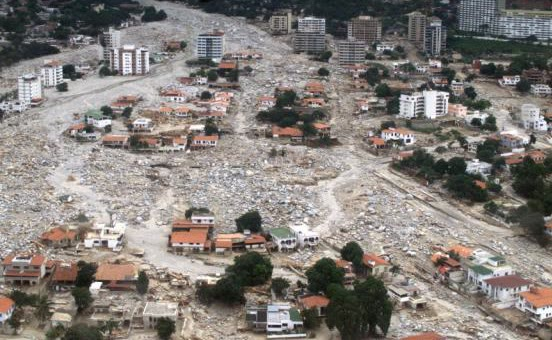
\includegraphics[width=0.62\linewidth]{images/book4/b2-28-caraballeda-debris-flow.jpg}
\par\smallskip{\small Dépôts de \omterm{def:b2:geological-hazards:slope}{lave torrentielle} sur le cône de Caraballeda, sur la côte du Venezuela,
après la tempête de décembre 1999~: les écoulements ont quitté le chenal principal et enseveli la
ville sous des blocs. Photographie~: Lawson Smith, U.S. Army Corps of Engineers (domaine public).}
\end{omfigure}
% ledger: photo:b2-28-caraballeda, vargas:caraballeda

\section{Tsunamis}\label{sec:b2:geological-hazards:tsunamis}

Un tsunami engendré par le soulèvement brutal du fond marin a une longueur d'onde
de quelques dizaines à quelques centaines de kilomètres, bien plus que la profondeur
de l'océan. C'est une onde longue, et sa vitesse ne dépend que de la profondeur.

\begin{proposition}[Ondes longues]\label{prop:b2:geological-hazards:long-waves}
Une onde de gravité de surface dont la longueur d'onde est beaucoup plus grande que la profondeur $h$
de l'eau se propage à $c = \sqrt{gh}$, quelle que soit sa longueur d'onde. Là où elle avance lentement
vers une eau moins profonde sans se réfléchir ni déferler, son amplitude $A$ croît comme $h^{-1/4}$.
\end{proposition}

\begin{proof}
La relation de dispersion donne la vitesse de phase $c = \omega/k = \sqrt{(g/k)\tanh(kh)}$. Pour une onde longue
$kh = 2\pi h/\lambda \ll 1$, et $\tanh(kh) \approx kh$, donc $c = \sqrt{gh}$, indépendante de
$k$~: les ondes longues ne se dispersent pas. L'énergie de l'onde par unité d'aire de surface de la mer est $\frac12
\rho g A^2$, et elle se propage à $c$. Si aucune énergie n'est réfléchie ou perdue, le flux $\frac12\rho g A^2
c$ à travers toute section reste le même le long du trajet~: $A^2 \sqrt{h}$ est constant, et $A \propto
h^{-1/4}$.
\end{proof}

Sur \qty{4000}{m} d'eau, un tsunami se propage à \qty{198}{m.s^{-1}}, soit
\qty{713}{km/h}~; sur \qty{5000}{m}, \qty{797}{km/h}, le « plus de 800 km/h » annoncé par les services
d'alerte. Près du rivage, dans \qty{10}{m} d'eau, il ralentit à \qty{36}{km/h} ; son front
est rattrapé par l'eau qui le suit, l'onde se raccourcit et se raidit, et sa hauteur croît.
% ledger: nws:tsunami-speed

\begin{definition}[Hauteur de run-up]\label{def:b2:geological-hazards:tsunami}
La \emph{hauteur de run-up}\index{hauteur de run-up} (remontée du tsunami) en un point de la côte est la
hauteur, au-dessus du niveau de la mer à cet instant, du point le plus élevé du terrain que l'eau atteint
à l'intérieur des terres. La distance horizontale entre le rivage et ce point est la distance d'inondation.
\end{definition}

Des équipes de relevé mesurent les run-up à partir des marques laissées par l'eau, des lignes de débris et des
dégâts relevés après chaque tsunami. La base mondiale des tsunamis compte \num{2177} observations de run-up pour
le tsunami de l'océan Indien du 26 décembre 2004, engendré par un séisme de magnitude 9.1 au large de Sumatra,
avec une hauteur d'eau maximale de \qty{50.9}{m}, et \num{6429} pour le tsunami du 11 mars 2011 au large de
Honshu, également de magnitude 9.1, avec un maximum de \qty{39.3}{m}. Ces deux tsunamis ont tué \num{227899} et
\num{18423} personnes. À Banda Aceh, l'eau a atteint le milieu du deuxième étage de la mosquée située en contrebas.
% ledger: ncei:tsu-2004, ncei:tsu-2011, usgs:aceh-mosque

\begin{omfigure}
\centering
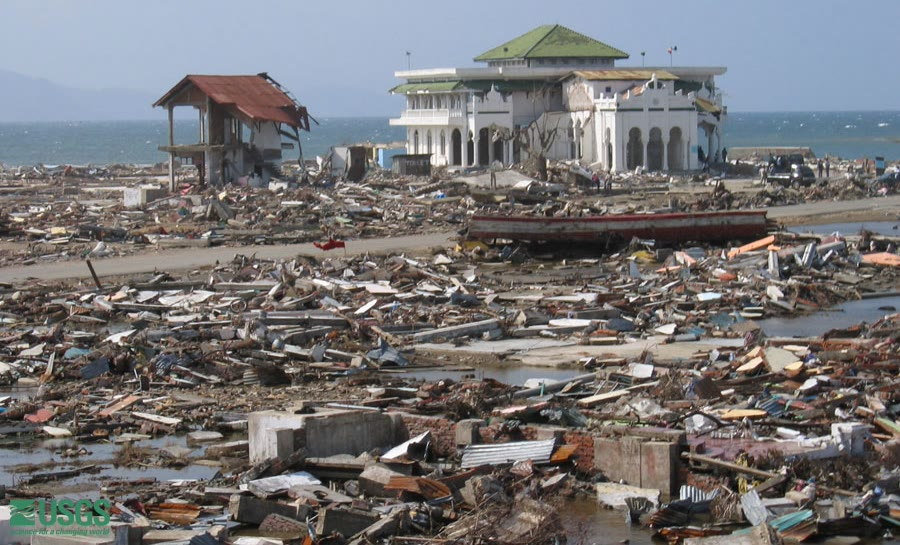
\includegraphics[width=0.62\linewidth]{images/book4/b2-28-aceh-mosque-tsunami.jpg}
\par\smallskip{\small Banda Aceh, Sumatra, le 21 janvier 2005, après le tsunami
du 26 décembre 2004~: une mosquée se dresse au milieu des décombres des bâtiments
qui l'entourent. Photographie~: U.S. Geological Survey (domaine public).}
\end{omfigure}
% ledger: photo:b2-28-aceh

\section{Crues}\label{sec:b2:geological-hazards:floods}

\begin{definition}[Courbe de fréquence des crues]\label{def:b2:geological-hazards:flood}
La \emph{courbe de fréquence des crues}\index{courbe de fréquence des crues} d'un cours d'eau
à une station de jaugeage est la courbe du débit de pointe annuel en fonction de sa \omterm{def:b2:geological-hazards:return}{période
de retour}, ou de sa probabilité annuelle de dépassement, construite à partir de la série
des pics annuels de la station et prolongée en général par une loi de probabilité ajustée.
\end{definition}

La formule de rang des volumes du secondaire place les points de la courbe. Elle a une raison.

\begin{proposition}[Position de tracé de Weibull]\label{prop:b2:geological-hazards:weibull}
Soient $n$ pics annuels indépendants tirés d'une même loi continue, et
$G(x)$ la probabilité qu'un pic annuel dépasse $x$. Le pic de rang $m$, compté à partir du plus grand,
a une \omterm{def:b2:geological-hazards:poisson}{probabilité de dépassement} moyenne $m/(n + 1)$, de sorte qu'il est placé à $T = (n +
1)/m$.
\end{proposition}

\begin{proof}
$U = G(X)$ est uniforme sur $[0, 1]$ pour une loi continue, et $G$ est décroissante, donc le $m$-ième plus grand pic
correspond au $m$-ième plus petit de $n$ variables uniformes indépendantes
$U_{(m)}$. Sa densité vaut $f(u) = \frac{n!}{(m-1)!\,(n-m)!}u^{m-1}(1-u)^{n-m}$ : l'une des $n$ valeurs en $u$
$m - 1$ en dessous et $n - m$ au-dessus. Avec l'intégrale bêta $\int_0^1 u^{p}(1-u)^{q}\,\mathrm{d}u
= p!\,q!/(p + q + 1)!$,
\begin{equation*}
\mathbb{E}[U_{(m)}] = \frac{n!}{(m-1)!\,(n-m)!}\cdot\frac{m!\,(n-m)!}{(n+1)!} = \frac{m}{n+1}. \qedhere
\end{equation*}
\end{proof}

Le plus grand pic d'un enregistrement de 30 ans est donc placé à 31 ans, et rien dans l'enregistrement ne fixe
la crue centennale. Pour l'atteindre, on ajuste les pics par une loi des extrêmes, souvent celle de Gumbel,
$\Pr(\text{pic} \leq x) = \exp\bigl(-e^{-(x - u)/\alpha}\bigr)$, dont la crue de $T$ ans est $x_T = u
- \alpha\ln\bigl(-\ln(1 - 1/T)\bigr)$~: une droite face à $-\ln(-\ln(1 - 1/T))$, extrapolée
au-delà de l'enregistrement, avec un risque qui croît avec la distance.

\section{Surveillance et alerte précoce}\label{sec:b2:geological-hazards:warning}

\begin{definition}[Système d'alerte précoce]\label{def:b2:geological-hazards:warning}
Un \emph{système d'alerte précoce}\index{système d'alerte précoce} est un dispositif
intégré de surveillance de l'aléa, de prévision, d'évaluation du risque, de communication
et de préparation, qui permet d'agir à temps avant un événement dangereux. Il
réunit quatre éléments~: la connaissance du risque~; la détection, la surveillance
et la prévision de l'aléa~; la diffusion des alertes~; et la préparation à réagir.
\end{definition}
% ledger: undrr:ews

La physique fixe le délai que peut donner chaque alerte. On ne peut pas devancer les ondes sismiques, mais les
ondes S, les plus dommageables, se propagent à environ \qty{3.2}{km.s^{-1}} dans la croûte supérieure, contre
\qty{5.8}{km.s^{-1}} pour les ondes P : une alerte calculée à partir des premières ondes P enregistrées près de
l'épicentre atteint une ville avant les ondes S, de $d(1/3.2 - 1/5.8) = \qty{0.14}{s}$ par kilomètre de distance
$d$, moins le temps de détection et de calcul. Une ville située à \qty{100}{km} gagne au plus \qty{14}{s}~; près
de la source, une zone aveugle n'en gagne aucun (voir l'\cref{exo:b2:geological-hazards:12}). Un tsunami traversant
\qty{100}{km} de mer de \qty{2000}{m} de profondeur met 12 minutes~; à travers un océan, il met des heures. En 2011,
l'alerte japonaise a été émise environ trois minutes après le séisme, mais sur une magnitude estimée trop basse,
car les instruments ont saturé~; elle a été mise à jour avec les données d'une bouée GPS au large environ 28 minutes
plus tard. Les enregistreurs de pression en eau profonde, qui convertissent la pression sur le fond marin toutes
les 15 secondes en une hauteur de la surface de la mer, signalent désormais par satellite le passage des tsunamis.
% ledger: data:prem, jma:warning, ndbc:dart
% values: 0.1401 s/km, 14.0 s at 100 km; 140 m/s over 2000 m, 11.9 min per 100 km (calc/ch28.py)

\begin{inthefield}[Suivre une pente qui se déplace]
Sur une pente connue pour fluer, les équipes de surveillance installent des instruments qui mesurent les
variables de l'équation de la pente infinie. Des piézomètres dans des forages enregistrent la pression
interstitielle sur la surface de glissement~; des tubes inclinométriques, lus à intervalles de profondeur,
montrent où le sol se courbe et à quelle vitesse~; des stations GNSS et des extensomètres enregistrent le
mouvement de la surface~; un pluviomètre enregistre le déclencheur. Les équipes comparent le mouvement à la
pluie et à la pression de l'eau, saison après saison, et cherchent l'accélération qui précède la rupture.
\end{inthefield}

\section*{Exercices}\label{sec:b2:geological-hazards:exercises}

Données pour les exercices, sauf indication contraire~: $g = \qty{9.81}{m.s^{-2}}$~; poids
volumique de l'eau \qty{9.81}{kN.m^{-3}}~; la GMPE \eqref{eq:b2:geological-hazards:gmpe}
sur rocher ($G_B = G_C = 0$), $\sigma = 0.230$~; vitesses des ondes P et S dans la croûte
supérieure de 5.8 et \qty{3.2}{km.s^{-1}}. Arrondir à trois chiffres significatifs.
% ledger: bjf93:pga, data:prem

\begin{exercise}[$\star$]\label{exo:b2:geological-hazards:1}
Dans le modèle de Poisson, (a) calculer la probabilité d'au moins une crue centennale en 30 ans~;
(b) calculer la probabilité qu'un siècle s'écoule sans crue centennale~; (c) trouver la \omterm{def:b2:geological-hazards:return}{période
de retour} du mouvement dont la \omterm{def:b2:geological-hazards:poisson}{probabilité de dépassement} en 50 ans est de \qty{5}{\percent}.
\end{exercise}

\begin{exercise}[$\star$]\label{exo:b2:geological-hazards:2}
Deux villes sont exposées à de fortes secousses. Dans la ville A, celles-ci surviennent à un rythme
d'une fois en 200 ans et détruiraient \qty{2}{\percent} de ses 5000 bâtiments~; dans la ville B, une
fois en 50 ans, détruisant \qty{10}{\percent} de ses 800 bâtiments. (a) Calculer le nombre attendu de
bâtiments détruits par an dans chaque ville. (b) Déterminer quelle ville présente le plus grand risque,
bien qu'elle ait la plus faible \omterm{def:b2:geological-hazards:risk}{exposition}. (c) Identifier lequel des trois facteurs fait la différence.
\end{exercise}

\begin{exercise}[$\star$]\label{exo:b2:geological-hazards:3}
(a) Calculer la vitesse d'un tsunami au-dessus de profondeurs de 4000, 200 et \qty{10}{m}.
(b) Calculer le temps qu'il met pour traverser \qty{1500}{km} d'océan de \qty{4000}{m}
de profondeur. (c) Trouver à quelle profondeur il se déplacerait à \qty{800}{km/h}.
\end{exercise}

\begin{exercise}[$\star$]\label{exo:b2:geological-hazards:4}
Un sable sec sans cohésion, d'angle de frottement $\varphi' = \ang{33}$, forme une longue pente.
(a) Calculer son \omterm{def:b2:geological-hazards:slope}{coefficient de sécurité} à \ang{25}. (b) Trouver la pente la plus raide qu'il peut
former. (c) La pente se sature d'eau, la nappe affleurant en surface, avec une infiltration parallèle
à celle-ci, de sorte que $r_u = \gamma_w\cos^2\beta/\gamma$, avec $\gamma = \qty{20}{kN.m^{-3}}$.
Montrer que $F = (1 - \gamma_w/\gamma)\tan\varphi'/\tan\beta$ et le calculer à \ang{25}.
\end{exercise}

\begin{exercise}[$\star\star$]\label{exo:b2:geological-hazards:5}
Le catalogue mondial compte 696 séismes de magnitude au moins 7 sur les 50 ans 1976--2025,
et l'intervalle moyen entre eux est de 26.2 jours. (a) Calculer leur taux annuel
moyen. (b) Dans le modèle de Poisson, calculer la probabilité qu'il s'écoule 30 jours
sans en voir un~; comparer avec la fraction observée d'intervalles plus longs que 30
jours, 0.304. (c) Calculer la probabilité d'au moins un séisme en une semaine donnée.
\end{exercise}

\begin{exercise}[$\star\star$]\label{exo:b2:geological-hazards:6}
(a) Calculer la PGA médiane d'un séisme de magnitude 6.5 sur rocher à $d = 0$, 10, 30 et \qty{100}{km}.
(b) Calculer ce qu'elle serait à \qty{10}{km} sur un site de classe C. (c) Déterminer entre quelles
valeurs se situe la PGA sur rocher à \qty{10}{km} avec une probabilité d'environ \qty{68}{\percent}.
\end{exercise}

\begin{exercise}[$\star\star$]\label{exo:b2:geological-hazards:7}
Les pics annuels d'un cours d'eau sur 12 ans étaient, en \unit{m^3.s^{-1}}~: 212, 148, 305, 176,
251, 133, 188, 420, 160, 229, 195, 268. (a) Donner les \omterm{def:b2:geological-hazards:return}{périodes de retour} des quatre plus grands.
(b) Estimer la crue décennale en interpolant linéairement en $\ln T$ entre les deux plus grands.
(c) Expliquer pourquoi cet enregistrement ne peut rien dire de fiable sur la crue centennale.
\end{exercise}

\begin{exercise}[$\star\star$]\label{exo:b2:geological-hazards:8}
Pour un volcan agité, l'observatoire estime~: agitation magmatique 0.6~; éruption si magmatique 0.4~;
\omterm{def:b2:eruptive-styles:regimes}{éruption explosive} si éruption 0.5~; une coulée pyroclastique atteignant une vallée donnée si explosive
0.3. (a) Calculer la probabilité d'une coulée pyroclastique dans la vallée. (b) Calculer la probabilité
d'une éruption, et celle d'une éruption sans coulée dans la vallée. (c) De nouvelles données de
déformation portent la probabilité d'une éruption, si l'agitation est magmatique, à 0.7. Mettre à jour (a).
\end{exercise}

\begin{exercise}[$\star\star$]\label{exo:b2:geological-hazards:9}
Un sol sec de $c' = \qty{8}{kPa}$, $\varphi' = \ang{30}$ et $\gamma = \qty{19}{kN.m^{-3}}$
repose sur une pente de \ang{35}. (a) Calculer l'épaisseur $z_c$ à laquelle $F = 1$. (b)
Calculer $F$ pour une couche de \qty{2}{m} d'épaisseur. (c) La même couche devient saturée,
la nappe affleurant en surface, avec $r_u = \gamma_w\cos^2\beta/\gamma$. Calculer $F$.
\end{exercise}

\begin{exercise}[$\star\star\star$]\label{exo:b2:geological-hazards:10}
(a) Montrer que le modèle de Poisson est sans mémoire~: la probabilité de n'avoir aucun événement dans $[s, s + t]$,
sachant qu'il n'y en a aucun dans $[0, s]$, vaut $e^{-t/T}$, quel que soit $s$. (b) Une faille a une \omterm{def:b2:geological-hazards:return}{période de
retour} de 475 ans pour ses grands séismes et n'en a pas eu depuis 400 ans. Calculer, dans le modèle, la probabilité
d'un tel séisme dans les 50 prochaines années. (c) Le rebond élastique du volume de première année suggère que la
probabilité devrait plutôt croître avec le temps écoulé depuis le dernier séisme. Identifier quelle hypothèse du modèle
de Poisson il contredit, et expliquer pourquoi les cartes d'aléa conservent le modèle pour les sources surfaciques.
\end{exercise}

\begin{exercise}[$\star\star\star$]\label{exo:b2:geological-hazards:11}
Un tsunami d'amplitude \qty{0.5}{m} et de période 20 minutes traverse un océan de \qty{4000}{m} de
profondeur. (a) En utilisant l'argument de flux d'énergie de la proposition sur les ondes longues,
calculer son amplitude dans \qty{10}{m} d'eau. (b) Calculer sa longueur d'onde aux deux profondeurs. (c)
Donner deux raisons pour lesquelles la remontée à la côte peut différer fortement de cette estimation.
\end{exercise}

\begin{exercise}[$\star\star\star$]\label{exo:b2:geological-hazards:12}
Un \omterm{def:b2:geological-hazards:warning}{système d'alerte précoce} sismique émet une alerte 4 secondes après l'arrivée de l'onde P à
sa station la plus proche de l'épicentre, à \qty{10}{km}. Négliger la profondeur de la source.
(a) Calculer à quel moment l'alerte est émise après le séisme. (b) Calculer combien de secondes
avant l'onde S une ville située à \qty{50}{km} de l'épicentre reçoit l'alerte, et une ville
à \qty{100}{km}. (c) Trouver le rayon de la zone aveugle, où l'onde S arrive avant l'alerte.
\end{exercise}

\begin{problem}[{Problème du week-end --- Une ville entre une faille et une pente}]\label{pb:b2:geological-hazards:1}
Une ville sur rocher se trouve à \qty{10}{km} d'une zone source~; tous ses séismes sont pris à
$d = \qty{10}{km}$. Leur récurrence est $\log_{10} N(\geq M) = 4.0 - 1.0\,M$ par an pour $M \geq 5$,
tronquée à $M_{\max} = 7.5$. La secousse suit la GMPE \eqref{eq:b2:geological-hazards:gmpe} avec
$\sigma = 0.230$. Au-dessus de la ville, une couche de sol de \qty{3}{m} d'épaisseur repose sur une
pente de \ang{30}, avec $\gamma = \qty{19}{kN.m^{-3}}$, $c' = \qty{4}{kPa}$ et $\varphi' = \ang{34}$~;
l'eau a un poids volumique de \qty{9.81}{kN.m^{-3}}. Arrondir à trois chiffres significatifs.

\noindent\textbf{Partie I --- Récurrence.}
\begin{enumerate}
\item Calculer les taux annuels de séismes de magnitude
au moins 5, 6 et 7, en négligeant la troncature.
\item Donner les \omterm{def:b2:geological-hazards:return}{périodes de retour} correspondantes.
\item Avec la troncature, calculer le taux des séismes de magnitude
supérieure à 7.5, et celui des séismes compris entre 7 et 7.5.
\item Calculer les taux des classes de magnitude 5--6 et 6--7.
\item Calculer la probabilité d'au moins un séisme de magnitude 6 ou plus en 50 ans.
\item Même calcul pour une magnitude 7 ou plus.
\end{enumerate}

\noindent\textbf{Partie II --- Mouvement du sol au niveau de la ville.}
\begin{enumerate}[resume]
\item Calculer $r$, et le terme de distance $-0.778\log_{10} r$.
\item Représenter les trois classes par les magnitudes 5.5, 6.5 et 7.25. Calculer
la médiane de $\log_{10}\mathrm{PGA}$ et la médiane de la PGA de chacune.
\item Calculer la PGA dépassée avec une probabilité de \qty{16}{\percent} par une magnitude 6.5.
\item Calculer la probabilité qu'une magnitude 6.5 produise plus de \qty{0.3}{g}.
\item Calculer la médiane de la PGA du plus grand séisme possible.
\end{enumerate}

\noindent\textbf{Partie III --- La courbe d'aléa.}
\begin{enumerate}[resume]
\item Calculer le taux annuel de dépassement de \qty{0.2}{g}, sommé sur les trois classes.
\item Même calcul pour \qty{0.3}{g}.
\item Même calcul pour \qty{0.4}{g}.
\item Calculer le taux annuel correspondant à \qty{10}{\percent} en 50 ans.
\item Déterminer entre lesquels des trois niveaux se situe ce taux.
\item En interpolant linéairement $\ln\lambda$ en fonction de $\ln a$, trouver
la PGA ayant une \omterm{def:b2:geological-hazards:poisson}{probabilité de dépassement} de \qty{10}{\percent} en 50 ans.
\item Déterminer quelles classes contribuent le plus au taux à
\qty{0.3}{g}, et commenter, à l'aide de la réponse à la question~11.
\end{enumerate}

\noindent\textbf{Partie IV --- La pente au-dessus de la ville.}
\begin{enumerate}[resume]
\item Calculer le \omterm{def:b2:geological-hazards:slope}{coefficient de sécurité} de la pente sèche.
  \item Le trouver lorsque la couche est saturée, la nappe affleurant en surface ($r_u =
        \gamma_w\cos^2\beta/\gamma$).
\item Calculer jusqu'à quelle fraction de l'épaisseur de la couche la nappe peut monter avant la rupture de la pente.
\item Dans une analyse pseudo-statique (admise), la secousse ajoute une force
horizontale $kW$. Calculer le $k$ critique de la pente sèche, pour lequel $F = 1$.
\item En prenant $k$ égal à la PGA en unités de $g$, déterminer quelle magnitude produit la
valeur critique comme médiane au niveau de la ville. Comparer avec la réponse à la question~17.
\item En résumé, calculer l'\omterm{def:b2:geological-hazards:psha}{accélération maximale du sol} ayant une probabilité
de \qty{10}{\percent} d'être dépassée en 50 ans au niveau de la ville.
\end{enumerate}
\end{problem}
